\problemname{The Eight Puzzle}

\begin{figure}[!h]
	\centering
	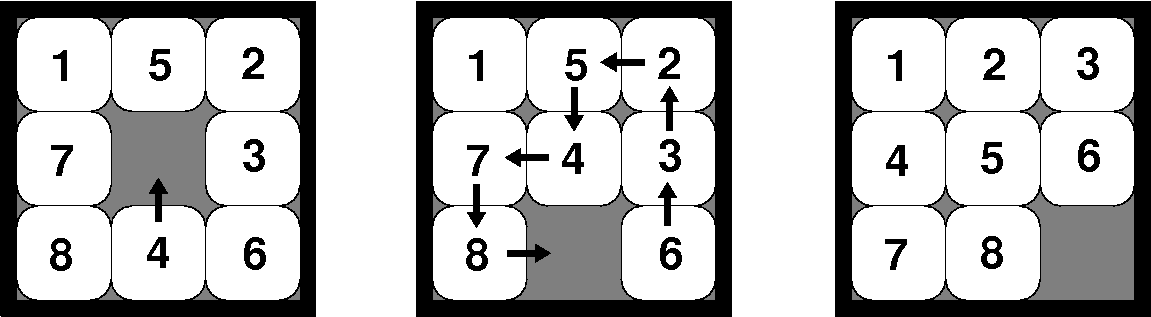
\includegraphics[width=0.55\textwidth]{figur}
	\caption{\emph{On the left, the starting position in the first example. The arrow shows the first move. The middle image shows the position after the first move and the arrows indicate the remaining seven moves needed to reach the final position shown on the right.}}
\end{figure}


\emph{The Eight Puzzle} (a younger sibling of the more well-known Fifteen Puzzle) is a type of puzzle consisting of eight square tiles in a frame. The tiles are numbered from $1$ to $8$. The frame fits $3\cdot3=9$ tiles, so there is one hole. A move consists of sliding an adjacent tile to the hole's position. Write a program that, given a starting position, computes the minimum number of moves needed to reach the ordered final position shown on the right in the figure above.

Hint: An arbitrary position is either unsolvable (which does not occur in the test cases) or has a solution with at most 31 moves.

\section*{Input}
The input consists of a line containing the tile number at each of the $9$ positions, or $0$ for the hole.
These are described by a line with $9$ integers, where the numbers are given in normal ``reading order'' (top row first, from left to right).
Each number between $0$ and $8$ will appear exactly once. In the given test cases, it will always be possible to reach the final position.

\section*{Output}
Output an integer: the minimum number of moves required to reach the final position from the given position.

\section*{Scoring}
Your solution will be tested on a set of test groups.
To earn points for a group, you must pass all test cases in that group.

\noindent
\begin{tabular}{| l | l | p{12cm} |}
  \hline
  \textbf{Group} & \textbf{Points} & \textbf{Constraints} \\ \hline
  $1$    & $40$          & There is a solution that uses at most 5 moves.  \\ \hline
  $2$    & $60$          & No additional constraints.  \\ \hline
\end{tabular}
